% \chapter{Some help on \LaTeX}
\chapter{Bibliography}

% This chapter contains examples of elements you will need. You can keep this and copy/paste from here whenever you need to use an instruction. Please read also the instructions for each element!

% \section{Text}
% \label{sec:text}

% When you write text and you want to make a new line, make \textit{two} new lines
% in the source; on the final PDF you will just see one. 

% \textbf{Do not} use:

% \begin{tight_enumerate}
%   \item \texttt{\textbackslash\textbackslash} to make a new line.
%   \item \texttt{\textbackslash newpage} to switch to a new page.
%   \item \texttt{\textbackslash noindent} to avoid the indentation of a new
%   paragraph.
% \end{tight_enumerate}

% \section{Figures}

% Figure \ref{fig:example} shows an example image. It describes various types of
% data on different levels of abstraction.

% \begin{figure}[ht]
% 	\centering
% 	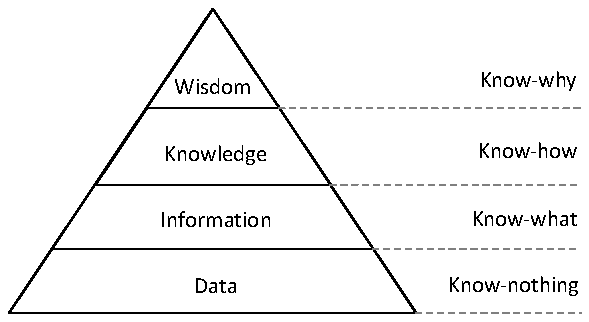
\includegraphics[scale=0.9]{img/example.pdf}
% 	\caption[Caption for the index]{Caption within the text \cite{Lauesen2002}.}
% 	\label{fig:example}
% \end{figure}

% Remember: 

% \begin{itemize}
%   \item Figures have to be referenced in the text using \texttt{\textbackslash
%   ref} and briefly explained. Do not worry if the image ends up on the following
%   page, probably there is no space to have it at the place where you inserted
%   it. 
%   \item Images should be vector images or saved with at least 600 dpi, so that
%   when printed they do not look blurry.
%   \item If the caption in the text and the index are the same, you can leave the
%   parameter for the caption for the index away, e.g., like
%   \texttt{\textbackslash caption\{Caption within the text.\}}
% \end{itemize}

% \textbf{Do not} use:

% \begin{tight_enumerate}
%   \item \texttt{\textbackslash begin\{figure\}[H!]} to force Latex to place a
%   figure where you want. Usually there is a good reason why a picture ends up
%   where it is positioned. Just refer to it with \texttt{\textbackslash ref} and
%   describe it. The reader is perfectly capable to find the image.
% \end{tight_enumerate}

% \section{Citations}
% You have to define reference material in a separate file called
% ``bibliography.bib''. Example of citations:
% \cite{Bass2012,Rubin2014,Dictionary1}. Have a look at \cite{rfc6824}.

% \section{Footnotes}
% Here is an example of a footnote\footnote{But do not use it too frequently :)}.
% Please use footnotes to provide the web site of any technology or product, e.g.,
% Microsoft Word\footnote{Microsoft Word,
% \url{http://office.microsoft.com/en-us/word}}, so that everyone knows what you
% are talking about.

% \section{Formulas}
% \LaTeX~is perfect for formulas: 
% \begin{equation}
% 	\label{equ:formula1}
% 	{\frac {d}{dx}}\arctan(\sin({x}^{2}))=-2\,{\frac {\cos({x}^{2})x}{-2+\left (\cos({x}^{2})\right )^{2}}}
% \end{equation}

% As you see in formula \ref{equ:formula1}, you can insert very nice formulas in
% your thesis too! Like figures, refer to the formula using \texttt{\textbackslash
% ref} and describe what the reader is seeing.

% \section{Tables}
% There are many ways to make a table, the table \ref{tab:tabExample} is a bit
% more complicated, but has many advantages, e.g., that you can have a table that
% breaks from one page to another.

% \begin{longtable}[c]{L{3cm}C{3cm}R{80pt}}
% \caption{Caption of the table within the text.} 
% \label{tab:tabExample} \\

% \toprule
% A & Header 2 & C \\
% \midrule
% \endfirsthead\longtableheader

% \toprule
% A & Header 2 & C \\
% \midrule
% \endhead\longtablefooter

% Left aligned & Center aligned & Right aligned \\
% Left aligned & Center aligned & Right aligned \\
% Left aligned & Center aligned & Right aligned \\
% Left aligned & Center aligned & Right aligned \\

% \end{longtable}

% Like for pictures and formulas, refer to the table using \texttt{\textbackslash
% ref} and describe what the reader is seeing.

% \textbf{Do not} use:

% \begin{tight_enumerate}
%   \item Vertical lines in a table
%   \item Double lines in a table
% \end{tight_enumerate}

% \section{Code}
% If you want to include code examples, you should use the \texttt{lstlisting}
% environment, as in listing \ref{lst:listing1}. 

% \begin{lstlisting}[caption=A listing example,label=lst:listing1]
% public ArrayList getList() {	
% 	ArrayList l = new ArrayList();
% 	Connection c = null;
% 	try {
% 		c = DatabaseTools.getConnection();
% 		Statement p = c.createStatement();
% 		ResultSet r = p.executeQuery("SELECT id, \"name\", readonly FROM \"group\" ORDER BY \"name\"");
% 		while (r.next()) {
% 			HashMap h = new HashMap();
% 			h.put("id", r.getString(1));
% 			h.put("name", r.getString(2));
% 			h.put("readonly", new Boolean(r.getBoolean(3)));
% 			l.add(h);
% 		}
% 	} catch (Exception e) {
% 		e.printStackTrace();
% 	} finally {
% 		if (c != null) {
% 			try {
% 				c.close();
% 			} catch (Exception e) {
% 				e.printStackTrace();
% 			}
% 		}
% 	}
	
% 	return l;
% }
% \end{lstlisting}

% Using the line numbers it is also easier to reference to them within the text.

% \section{Landscape}

% Sometimes, you need to show a picture or a table that requires a lot of space.
% To avoid that the text in the picture or table becomes unreadable, you can
% insert it in landscape mode, like the text on the next page.

% \begin{landscape}
% Some text in landscape mode.
% \end{landscape}
